\tocless\subsubsection{Transactions}

A database is a collection of data items that hold values. A database system (\textit{DBS}) is a tool comprised of software and hardware components that manages access to the underlying database. It allows its users to perform specific operations on the database items. Those can be summarized as being one of two kinds, reads and writes. In the following, we will use the notation \tread{x} to represent a read operation of the database item named \textit{x} while \twrite{x}{v} to depict a write operation which sets item \textit{x}'s value to \textit{v}. We will use the shorthand notation \twritee{x} to mean that some value is written to item $x$. Both the mentioned kind of operations are executed atomically \cite{ccontrol}. This means that the execution of a set of such operations appears to be sequential in terms of its constituents.

It is often the case that several operations are grouped together in order to make them behave as if they were a single unit of work. In such situations, database transactions are used: an ordered collection of operations. For example, considering a database for bank accounts, we consider a transfer of funds as a single operation from the user's point of view even if in reality the \textit{DBS} performs multiple sequential reads and writes to achieve the goal, as shown in Figure \ref{fig:transfer}. A transaction execution must provide guarantees on the well known \textbf{ACID} properties \cite{dbconcepts}, an acronym for:
\begin{enumerate}[ref=(\arabic*)]
\item \label{acid.a} Atomicity: all of the transaction's operations are executed or none of them; there is no possible partial execution of a transaction.
\item \label{acid.c} Consistency: an isolated execution of a transaction maintains the consistency constraints of the database. In our bank example, the property would be maintained when money is neither created nor destroyed as part of a transfer, but simply \textit{moved}.
\item \label{acid.i} Isolation: a transaction executes as if no other one is running in the \textit{DBS} at the same time. More generally, a given isolation level determines the correct behaviours of transactions that run concurrently. For example, serializability implies that any two transactions running in parallel believe that the other one has either finished before they started or it will start after they finished executing.
\item \label{acid.d} Durability: once a transaction has completed its work, all of its changes are kept in the database even if failures happen in the future.
\end{enumerate}

In order to maintain property \ref{acid.a}, a transaction needs to communicate the completion of its operations or its interruption in case of failure. This is done by introducing two new types of operation, namely commit and abort, which are notated \tcommit and \tabort respectively. In the case of an abort, the \textit{DBS} must roll-back the state of the database to what it was prior to the start of the transaction in order to undo the changes performed up to the failure point.

\begin{center}
\begin{tabular}{c@{\hskip 0.5in}c}
\begin{lstlisting}
BEGIN
	balance := R[a]
	W[a, balance-100]
	balance := R[b]
	W[b, balance+100]
	C
END
\end{lstlisting}
&
\begin{lstlisting}
BEGIN
	balance := R[a]
	W[a, balance-5000]
	A
END
\end{lstlisting}
\end{tabular}
\captionof{figure}{Two examples of transactions on the bank database. Note how the second one aborts due to a failure (potentially insufficient funds).}
\label{fig:transfer}
\end{center}

Following the explanation in \cite{ccontrol}, we formally define a transaction $T$ as the tuple $(\theta, \sqsubset)$ where $\theta$ is the set of all operations in $T$ and $\sqsubset$ is a partial order on $\theta$. The latter is defined as:
\[
	\theta \subseteq \left\lbrace op\ |\ op \in \lbrace \tread{x}^i, \twritee{x}^i \rbrace, x \in \pred{items}{db}, i \in \mathds{N} \right\rbrace \cup \left\lbrace \tcommit, \tabort \right\rbrace
\]
The set of operations, $\theta$, maintains the constraint $\left(\tcommit \in \theta \Leftrightarrow \tabort \notin \theta\right)$ while the ordering relation, $\sqsubset$, must satisfy the property that if the transaction contains an operation $t$ which is either a commit or an abort, then all operations must appear in a transaction before $t$. Formally,
\[
	\forall t \in \{\tcommit, \tabort\} \ldotp t \in \theta \Rightarrow \left( \forall op \in \theta \ldotp op \neq t \Rightarrow op \sqsubset t \right)
\]

Also, we state that, as part of a single transaction, any two operations that involve a particular item, with at least one of them being a write, must be ordered according to $\sqsubset$:
\begin{gather*}
	\forall x \in \pred{items}{db}, op, i, j \ldotp \left( op \in \left\lbrace \tread{x}^i, \twritee{x}^i \right\rbrace \land \lbrace op, \twritee{x}^j \rbrace \subseteq \theta \right) \\ \implies (\twritee{x}^j \sqsubset op \lor op \sqsubset \twritee{x}^j)
\end{gather*}
For the example in Figure \ref{fig:transfer} we would have the following transaction definition:
\begin{gather*}
\theta \equiv \left\lbrace \tmread{\texttt{a}}^1, \tmread{\texttt{b}}^2, \tmwritee{\texttt{a}}^3, \tmwritee{\texttt{b}}^4, \tcommit \right\rbrace
\\[0.4em]
\sqsubset\ \equiv \{ (\tmread{\texttt{a}}^1, \tmwritee{\texttt{a}}^3), (\tmread{\texttt{b}}^2, \tmwritee{\texttt{b}}^4), (\tmread{\texttt{a}}^1, \tcommit), (\tmread{\texttt{b}}^2, \tcommit), (\tmwritee{\texttt{a}}^3, \tcommit), (\tmwritee{\texttt{b}}^4, \tcommit) \}
\end{gather*}
This gives the \textit{DBS} the option to arbitrarily schedule the operations which are not ordered according to $\sqsubset$. In fact, under the mentioned example, one could invert the order of the two reads (or even run them in parallel) and still always get to the same final result. As we will see in section \ref{histories}, if a history is proven to be serializable, then we can guarantee valuable properties about it.

\tocless\subsubsection{Histories} \label{histories}

Modern database systems employ concurrency in order to run multiple transactions at the same time to achieve a higher performance and better operations throughput. On the downside, running operations in parallel on shared data items can lead to race conditions and a potential loss of two of the aforementioned ACID properties, consistency and isolation.

% In order to investigate the matter further, we will introduce some definitions which will prove useful.
The interleaving of operations which arises from a concurrent run of transactions, is referred to as a history. It records the order in which operations actually happen on the database and given that some of them could effectively execute in parallel, they are not totally ordered. A history $H$ \cite{ccontrol} is therefore a tuple $(\Theta, \pord)$ such that for a set of $n$ transactions $T_H = \left\lbrace T_i \right\rbrace_{i \in I}$, where $I = \{ i\ |\ 1 \leq i \leq n\}$, we have the operations set $\Theta$ and the partial order $\pord$ such that:
\[
	\begin{array}{c}
		\Theta \triangleq \bigcup_{i = 1}^{n} \theta_i\
		\text{ and }\
		\bigcup_{i = 1}^{n} \sqsubset_i\ \subseteq \pord
	\end{array}
\]
Let's also define two operations as conflicting if they both access the same data item and one of them is a write; formally we describe the property as:
\[
	\pred{conflict}{op_\alpha, op_\beta} \Leftrightarrow \left( op_\alpha \in \{ \tread{x}, \twritee{x} \} \land op_\beta = \twritee{x} \right) \lor \left( op_\alpha = \twritee{x} \land op_\beta \in \{ \tread{x}, \twritee{x} \} \right)
\]
We then require that all conflicting operations appearing in a history must be somehow ordered by $\pord$.
\[
	\forall op_\alpha, op_\beta \ldotp (\pred{conflict}{op_\alpha, op_\beta} \land\left\lbrace op_\alpha, op_\beta \right\rbrace \subseteq \Theta) \Rightarrow (op_\alpha \pord op_\beta \lor op_\beta \pord op_\alpha)
\]
When considering a history $H_{total}$ which is a total order over the operations of its transactions, we can refer to it simply by $\twritee{x}_i^1, $ $\twritee{y}_j^1, $ $\tcommit_i, $ $\tread{x}_j^2, $ $\twritee{x}_j^3, $ $\tcommit_j$ for example.

For every history $H = (\Theta, \pord)$ we can compute the group of transactions which committed as part of it as the set:
\[
	\pred{committed}{H} \triangleq \{ T_i\ |\ \tcommit_i \in \Theta \}
\]
This definition will aid us in describing a fundamental structure for the analysis of histories, the precedence or serialization graph. The latter allows to establish relationships between the transactions committing their operations as part a history. We can now build a history's precedence graph $G(H) = (V, E)$ where the set of vertices $V = \pred{committed}{H}$ includes all committed transactions in $H$ and an edge $(T_i, T_j)$ is in $E$, if transaction $T_i$ has an operation which is ordered before one in $T_j$ and the two are conflicting \cite{dbconcepts}. Formally, the set of edges is defined as:
\[
	E \triangleq \{ (T_i, T_j)\ |\ i \neq j \land \exists op_\alpha, op_\beta \ldotp op_\alpha \in \theta_i \land op_\beta \in \theta_j \land op_\alpha\ \pord\ op_\beta \land \pred{conflict}{op_\alpha, op_\beta} \}
\]

In Figure \ref{fig:exPrecGraph} we can see a concrete instance of a history with $3$ transactions and its corresponding precedence graph. Note that the graph's nodes include the three transactions since they all commit as part of $H$. On top of this, the edge from $T_1$ to $T_2$ is justified by pair the conflicting operations $(\tmread{x}_1^1, \tmwritee{x}_2^2)$, while the one from $T_1$ to $T_2$ by the pair $(\tmread{y}_1^2, \tmwritee{y}_3^1)$.

\begin{center}
\begin{tikzpicture}[->, semithick]
\node (1) {$T_1$};
\node (2) [right = 0.5cm of 1] {$T_2$};
\node (3) [right = 0.5cm of 2] {$T_3$};

\path
(1) edge node {} (2)
(1) edge [bend left] node {} (3);
\end{tikzpicture}
\\[0.4em]
$H \equiv \tmread{x}_1^1, \tmread{x}_2^1, \tmread{y}_1^2, \tmwritee{x}_2^2, \tcommit_2, \tmwritee{y}_3^1, \tcommit_1, \tcommit_3$
\captionof{figure}{An example history with its corresponding precedence graph.}
\label{fig:exPrecGraph}
\end{center}

A history $H_i$ is said to be equivalent to another history $H_j$ \cite{ccontrol}, when they have the same set of transactions which committed as part of them, and they order conflicting operations in the same way. We formally write $H_i \equiv H_j$, and this holds if and only if:
\begin{gather*}
	\pred{committed}{H_i} \equiv \pred{committed}{H_j} \\
	\land \forall op_\alpha, op_\beta \ldotp (\pred{conflict}{op_\alpha, op_\beta} \land \left\lbrace op_\alpha, op_\beta \right\rbrace \subseteq \Theta_i) \Rightarrow (op_\alpha\ \pord_i\ op_\beta \Leftrightarrow op_\alpha\ \pord_j\ op_\beta)
\end{gather*}
The latter condition is necessary because the result of a concurrent execution of a set of transactions only depends upon the relative ordering of conflicting operations. We describe a history as serial if all of its constituent transactions are run one after the other, without an interleaving of their operations. Such histories guarantee the highest possible database isolation. It is possible to further state that any history $H$ is serializable if and only if it is equivalent to some serial history $H'$. The serializability theorem states that any history $H$, such that its precedence graph $G(H)$ contains no cycles, is serializable \cite{ccontrol}.

\tocless\subsubsection{Anomalies and Isolation Levels}

The \textsc{Ansi/Iso Sql-92} standard \cite{ansi92} defines a set of different transaction isolation levels based on partial histories they allow as part of the possible interleavings. We will call these sequences of actions phenomena. The original standard describes 3 of such phenomena, while Berenson et al. \cite{isolationansi} add an extra one \ref{ansi:0} for completeness.

\begin{enumerate}[label=(\textbf{P\arabic*})]\addtocounter{enumi}{-1}
\item \label{ansi:0} A \textbf{dirty write} appears when a transaction $T_i$ writes to a data item and, before it commits or aborts, another transaction $T_j$ writes to the same item. If any of $T_i$ and $T_j$ were to abort, it is not clear what value the item should contain.
\\
E.g. $H_{DW} \equiv \ldots \tmwritee{x}_i \ldots \tmwritee{x}_j \ldots$
\item We have the \textbf{dirty read} phenomenon in the case where transaction $T_i$ writes to an item, then, before it commits or aborts, another transaction $T_j$ reads that same data item. In fact if $T_i$ would abort after $T_j$ has already read, the latter would have retrieved a value for the item that never actually existed.
\\
E.g. $H_{DR} \equiv \ldots \twritee{x}_i \ldots \tread{x}_j \ldots$
\item A \textbf{non-repeatable read} happens when a transaction $T_i$ reads a data item which is later written to by another transaction $T_j$ that also commits. At this point, if $T_i$ is to read the same item again, it would either discover a new value or fail due to a removal.
\\
E.g. $H_{NR} \equiv \ldots \tread{x}_i \ldots \twritee{x}_j \ldots \tcommit_j \ldots$
\item The \textbf{phantom} phenomenon appears when transaction $T_i$ queries all data items satisfying a particular condition $\gamma$. Transaction $T_j$ then inserts some new items that satisfy $\gamma$. Now, if $T_i$ were to reproduce the initial query, it would see new items appear.
\\
E.g. $H_{P} \equiv \ldots \tmread{\gamma}_i \ldots \tmwritee{\gamma}_j \ldots \tmread{\gamma}_i \ldots$ here we abuse the transaction notation in the following way $\tmread{\gamma} \triangleq \left\lbrace x\ |\ x \in \pred{items}{db} \land \gamma(x) \right\rbrace$ and $\tmwritee{\gamma} \triangleq \exists x, v \ldotp \gamma(x) \land \tmwrite{x}{v}$.
\end{enumerate}

The listed definitions can be used to formulate the \textsc{Ansi} isolation levels as they appear in Table \ref{table:isolation}. The choice of how to concurrently run several transactions given by a $DBS$ allows clients to achieve a better performance or stronger consistency depending on how strict the isolation level is. In fact, allowing some of the phenomena can lead to failing constraint checks in the database.
\begin{center}
\captionof{table}{\textsc{Ansi} isolation levels and the phenomena they allow \cite{ansi92} \cite{isolationansi}.}
\def\arraystretch{1.4}
	\begin{tabular}{l|c c c c}
		\hline
		\textbf{Isolation Level} & \textbf{Dirty Write} & \textbf{Dirty Read} & \textbf{N-R Read} & \textbf{Phantom} \\
		\hline
		Read Uncommitted & $\times$ & \checkmark & \checkmark & \checkmark \\
		Read Committed & $\times$ & $\times$ & \checkmark & \checkmark \\
		Repeatable Read & $\times$ & $\times$ & $\times$ & \checkmark \\
		Serializable & $\times$ & $\times$ & $\times$ & $\times$ \\
		\hline
	\end{tabular}
\label{table:isolation}
\end{center}

A concrete example of how the presence of the described phenomena can lead to a lack of correctness is shown in Table \ref{table:inconsistent} where transactions run at the read committed level. Let's assume that $T_i$ is executed by a bank's agent that wants to read what percentage of the overall funds are held by customer $a$ and $T_j$ is directly performed by $a$ as a cash withdrawal from an ATM machine. The former would first read the balance of $a$ then sum the funds of all customers (in this case $a$, $b$, $c$) and perform a simple division. On the other hand, $T_j$ will first read the cash availability, then subtract $\$100$ and provide the money to the customer. Given the isolation level selected, a non-repeatable read appears as part of history $H$ as $T_j$ removes the money after $T_i$ has read the initial balance for $a$ and before it has computed the overall sum. Therefore the end result $(\texttt{b}\div\texttt{total})$ will be incorrect and larger than the actual one. Moreover, this is a consequence to the fact that $H$ is not serializable. We can show this by first noticing that there are two possible serial histories:
\begin{align*}
	H_1 &= \tmread{a}_1^1, \tmread{a}_1^2, \tmread{b}_1^3, \tmread{c}_1^4, \tcommit_1, \tmread{a}_2^1, \tmwritee{a}_2^2, \tcommit_2 \\[0.5em]
	H_2 &= \tmread{a}_2^1, \tmwritee{a}_2^2, \tcommit_2, \tmread{a}_1^1, \tmread{a}_1^2, \tmread{b}_1^3, \tmread{c}_1^4, \tcommit_1
\end{align*}
The conflicting operations that happen as part of the execution are the pairs $(\tmread{a}_1^1, \tmwritee{a}_2^2)$ and $(\tmread{a}_1^2, \tmwritee{a}_2^2)$. The relative order in which they appear in the histories we consider is expressed as follows:
\[
	\begin{array}{c}
		H: \tmread{a}_1^1\ \pord_H\ \tmwritee{a}_2^2\ \pord_H\ \tmread{a}_1^2
		\\[0.5em]
		\begin{array}{c c}
			H_1 : \tmread{a}_1^1\ \pord_{H_1}\ \tmread{a}_1^2\ \pord_{H_1}\ \tmwritee{a}_2^2\
			&\
			H_2 : \tmwritee{a}_2^2\ \pord_{H_2}\ \tmread{a}_1^1\ \pord_{H_2}\ \tmread{a}_1^2
		\end{array}
	\end{array}
\]
It is clear that the particular ordering of conflicts in $H$ is neither the same as the one in $H_1$, nor to the one in $H_2$. Therefore since $H$ is not equivalent to any of $H_1$ and $H_2$, it is clearly not serializable. A plausible solution for this kind of issue is to change the isolation level of the $DBS$ to repeatable read which forbids the presence of the culprit phenomenon.
\begin{center}
\captionof{table}{History $H$ showing a concurrent run of two transactions $T_i$ and $T_j$.}
\def\arraystretch{1.4}
\begin{tabular}{c|@{\hspace{15pt}} c @{\hspace{15pt}} c}
\hline
\textbf{Time $t$} & $T_i$ & $T_j$ \\
\hline
0 & \texttt{b} = $\tmread{a}_i^1$ & \texttt{c} = $\tmread{a}_j^1$ \\
1 & - & $\tmwrite{a}{\texttt{c}-100}_j^2$ \\
2 & - & \tcommit \\
3 & \texttt{total} = $\tmread{a}_i^2$ + $\tmread{b}_i^3$ + $\tmread{c}_i^4$ & - \\
4 & \tcommit & - \\
\hline
\end{tabular}
\label{table:inconsistent}
\end{center}

\tocless\subsubsection{Locking Protocols}

The most popular mechanism to enforce a particular isolation level is to use some form of locking. We can consider each data item $x \in \pred{items}{db}$ to be associated with a lock that manages the access to its value. When a transaction runs an operation which accesses $x$, it is required to hold the lock relative to the item. The exact synchronization structure used in this case is a read/write lock that works under two modes, a shared one and an exclusive one. The former allows multiple read operations to happen in parallel while the latter makes sure that there is only one write operation executing at any point in time. This way, execution blocking only happens when transactions perform concurrent conflicting operations on the same data item. In terms of notation, a transaction $T_i$ can lock an item using $\tlock{\kappa}{x}_i$ and unlock it with $\tunlock{\kappa}{x}_i$ where $\kappa \in \{ \tshared, \texclusive \}$ is the lock mode (shared or exclusive). If a transaction requests access to item $x$ and gets an immediate grant even if $x$'s lock is held by another transaction, we say that the two locks are compatible \cite{dbconcepts}. We define this property for lock modes as follows:
\[
	\pred{compatible}{\kappa, \kappa'} \iff (\kappa = \tshared \land \kappa' = \tshared)
\]

We can specify the usage of locks in a formal way by describing histories $H$ that arise from locking protocols. Given that all accesses to database items are well locked, we know that they must be guarded by the corresponding and appropriate locks which are later released, so:
\begin{gather*}
	\forall x, i \ldotp \left( \tmwritee{x}_i \in \Theta_H \implies \tlock{\texclusive}{x}_i\ \pord\ \tmwritee{x}_i\ \pord\ \tunlock{\texclusive}{x}_i \right) \\[0.3em]
	\land \left( \tmread{x}_i \in \Theta_H \implies \exists \kappa \ldotp \tlock{\kappa}{x}_i\ \pord\ \tmread{x}_i\ \pord\ \tunlock{\kappa}{x}_i \right)
\end{gather*}
On top of this, when that a transaction requests an already acquired and non-compatible lock, it must wait for the counterpart to release. This implies that as part of locking protocols' histories, we will see that:
\begin{gather*}
	\forall x, \kappa_a, \kappa_b, i, j \ldotp \\
	(i \neq j \land \lnot \pred{compatible}{\kappa_a, \kappa_b} \land \{ \tlock{\kappa_a}{x}_i, \tunlock{\kappa_a}{x}_i, \tlock{\kappa_b}{x}_j, \tunlock{\kappa_b}{x}_j \}\subseteq \Theta_H) \\
	 \implies (\tlock{\kappa_a}{x}_i\ \pord\ \tunlock{\kappa_b}{x}_j \lor \tlock{\kappa_b}{x}_j\ \pord\ \tunlock{\kappa_a}{x}_i)
\end{gather*}

Two-Phase-Locking (\tpl) is a concurrency control protocol which is vastly used in commercial $DBS$ products. In its base version, as the name suggests, each transaction $T_i$'s execution can be divided into two phases \cite{ccontrol}: a growing phase where $T_i$ sequentially acquires locks for all the data items it is going to access, and a shrinking phase that starts on the first lock release and will unlock all the items it holds, one after the other. According to \tpl, during the growing phase no locks are released, and once the shrinking phase has started, no locks are acquired. Formally, all histories that result from the use of \tpl\ will have an additional property in comparison to the ones already mentioned for locking protocols. In fact lock operations will be further ordered as to comply with the two phase separation:
\[
	\forall x, y, \kappa_a, \kappa_b, i \ldotp (\{ \tlock{\kappa_a}{x}_i, \tunlock{\kappa_b}{y}_i \} \subset \Theta_H \implies \tlock{\kappa_a}{x}_i\ \pord\ \tunlock{\kappa_b}{y}_i)
\]

A variation of the method is Conservative Two-Phase-Locking (\textsc{c2pl}) that works in a similar way with the key difference that all locks ever needed as part of a transaction are acquired before any read or write operation happens. As a consequence, we can state that all histories $H$ adhering to \textsc{c2pl} will be such that:
\[
	\forall x, op, \kappa, i \ldotp (op \neq \textsf{L} \land \{ \tlock{\kappa}{x}_i, op \} \subseteq \Theta_H) \Rightarrow \tlock{\kappa}{x}_i\ \pord\ op
\]
This is done primarily in order to prevent situations in which \tpl\ would exhibit deadlocks, since lock acquisitions can be done in some precise order that all transactions need to follow.

Another version of \tpl\ which is widely used inside concrete implementations is Strict Two-Phase-Locking (\stpl) which imposes a different kind of constraint. Specifically, it only allows transactions to release the locks they hold after they have either committed or aborted. Its histories follow the rules listed for standard \tpl\ and moreover they guarantee that:
\[
	\forall x, op, \kappa, i \ldotp (op \in \{ \tcommit_i, \tabort_i \} \land \{ \tunlock{\kappa}{x}_i, op \} \subset \Theta_H) \Rightarrow op\ \pord\ \tunlock{\kappa}{x}_i
\]
The Strong-Strict Two-Phase-Locking (\textsc{ss2pl}) protocol works by combining the two previous approaches in a way that all locking operations happen before any access to items and all unlocking operations appear after a transaction's commit or abort completion. We summarize the pecularities of the four variants of the protocol in Table \ref{table:2plvariants}. Gradual locking refers to a transaction acquiring locks for cells as it needs to, while the extreme version makes it obtain all needed locks before starting. Similarly, gradual unlocking releases locks whenever they are no longer needed (while still following the two phases rule) and, on the other hand, extreme unlocking only releases locks after a transaction has committed.
\begin{center}
\captionof{table}{Two-Phase-Locking variants' constraints.}
\setlength{\tabcolsep}{14pt}
\def\arraystretch{1.6}
\begin{tabular}{l|c c c c}
\hline
\textbf{Constraint} & \textsc{2pl} & \textsc{c2pl} & \textsc{s2pl} & \textsc{ss2pl} \\
\hline
Gradual Locking & \checkmark & $\times$ & \checkmark & $\times$ \\
Extreme Locking & $\times$ & \checkmark & $\times$ & \checkmark \\
Gradual Unlocking & \checkmark & \checkmark & $\times$ & $\times$ \\
Extreme Unlocking & $\times$ & $\times$ & \checkmark & \checkmark \\
\hline
\end{tabular}
\label{table:2plvariants}
\end{center}

\tocless\subsubsection{Serializability \& Transactional Models}

\label{sec:serTransMod}

The theory for database transactions that we introduced so far has recently had a large number of applications to the more general context of programming languages. Transactions are being effectively used in the latter to provide an overall simplification to shared-memory concurrency. Popular commercial programming languages provide syntactic constructs to embed a chunk of code into an atomic transaction. This allows to free programmers from the burden of mantaining the fictional atomicity of operations, and delegate everything to the language implementation. We explore two models of transactions in this setting.

\paragraph{Push/Pull Model}
The model of transactions described in \cite{pushPull} is presented as a general theory of serializability, that abstracts away all of the algorithm and implementation details, in order to find a compact set of operations used in the vast majority of cases. The model does not use a concrete machine state, i.e. a global storage or memory heap, to track the effect of transactions' operations such as writes. Instead, it assigns a local \textit{log} of operations to each transaction and considers a unique shared log, which records the history of all globally visible operations. The semantics allow transactions to \textsc{Push} or \textsc{Unpush}, in order to share their local effects with the global log or to recall them from it. Conversely, they can \textsc{Pull} an operation from the shared log into their local view, together with detangling from one through an \textsc{Unpull}. These two types of actions can be seen as reading or \textit{forgetting} a read from the global storage. The framework comes with a proof of serializability within the semantic model, meaning that once users map their algorithms to push \textit{Push/Pull} semantic rules, they obtain a proof of serializability as a consequence.

\paragraph{Semantics for Transactions} The work done in \cite{semanticsTransactions} presents a set of formal languages which are able to describe particular behaviours that arise from the use of transactions within a programming language. Those are defined in terms of small-step operational semantics that allow the interleaving of parallel operations. They are high-level in order not to appear too complicated to the eyes of a programmer, while still detailed enough to express the required features. The languages of the \textsf{AtomsFamily} are listed here, in increasing order of consistency strictness:
\begin{enumerate}
	\item \label{highLevel.1} As part of \textsf{StrongBasic} only one single thread is allowed to execute a transaction at one time. On top of this, a running transaction cannot spawn a new thread and other parallel threads cannot read or write memory cells from the global heap. This is the strongest and simplest of the languages.
	
	\item The \textsf{StrongNestedParallel} language is an extension of the one described in (\ref{highLevel.1}). It allows to spawn threads within transactions in multiple ways. The expression $\mathsf{spawn_{oc}}$, \textit{spawn on commit}, is allowed anywhere in a program, but if included in a transaction, the spawned thread only reduces once the transaction completed. $\mathsf{spawn_{ip}}$, \textit{internally parallel}, is only allowed within a transaction and the latter can only commit once the spawned thread completed.
	
	\item \label{highLevel.2} \textsf{Weak} is a modified version of the language in \ref{highLevel.1} with the removal of the nontransactional code constraint. As a consequence, threads running in parallel to a transaction can access the shared heap through nontransactional commands.
	
	\item Finally, the \textsf{WeakUndo} language has all the features of the one in (\ref{highLevel.2}) together with the possibility for a transaction to abort, undo all of the heap updates and retry.
\end{enumerate}

\paragraph{Consistency Models} Cerone et al. \cite{ceroneConcur15} define a general framework for transactional consistency models within the context of distributed systems, in particular of geo-replicated databases. In this scenario, guaranteeing that the database behaves as if transactions get executed serially is often too slow, or unfeasible due to network failures. This is the main reason why weaker consistency guarantees are taken into account, which allows the occurrence of behaviours prohibited by serializability. The framework itself enables to uniformly specify a variety of such models by taking an axiomatic approach, with the goal of reasoning about databases at a high level of abstraction. What is key in finding common ground among a number of consistency models is the property of atomic visibility. This states that it is guaranteed that all or none of the effects of a transaction are visible to others. Replicated database systems typically enforce this behaviour. The crucial difference is then to understand and analyse when the effects become visible.

As part of the framework, reasoning happens at the level of abstract database executions, that are a structures of events with particular relations on them. Each introduced consistency model is specified through consistency axioms that restrict the possible abstract executions. We will go through the high-level details of a two of such models to understand how they are generally developed.

The baseline model is \textbf{Read Atomic}, which is defined through two axioms. The internal consistency axiom, \textsc{Int}, ensures that, as part of the body of a transaction, the value read from a database item $x$ is equivalent to the last value written to $x$ or the last value read from it. On the other hand, the external consistency axiom, \textsc{Ext}, enforces that any time a transaction $T$ reads a value from item $x$ before it writes to it, it will obtain a value which was written to $x$ by transactions preceding $T$. In the case where no transaction wrote to $x$, the default value of $0$ will be returned.

The \textit{precedence} between transactions is given by the visibility relation, \textsf{VIS}. We write $T_1 \xrightarrow{\mathsf{VIS}} T_2$ in order to express that $T_2$'s internal operations can be influenced by $T_1$'s effect on the database. Another fundamental relation of abstract executions is arbitration, \textsf{AR}, which is defined on transactions. The meaning of $T_1 \xrightarrow{\mathsf{AR}} T_2$ is that transaction $T_2$'s version of database items supersedes the one written to by $T_1$.

The adoption of the \textbf{Read Atomic} model leads to a variety of anomalies including the one of causality violation, an example of which is graphically shown in Figure \ref{fig:causVio}. In order to forbid this kind of behaviour we are required to strengthen the consistency model with a new axiom, \textsc{TransVis}. Causal consistency will in fact be obtained by enforcing the \textsf{VIS} to be transitive. It follows that the effects of transactions ordered by \textsf{VIS} are observed by others in this same order.
\begin{center}
	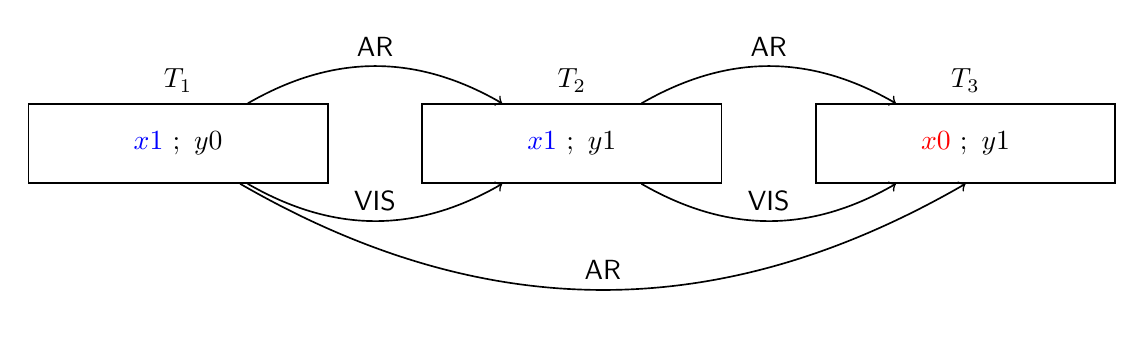
\begin{tikzpicture}[->, semithick]
		\tikzset{
		    trans/.style= {rectangle, draw=black, color=black, minimum width=3.8cm, minimum height=1cm},
		    vis/.style= {above, black!5!black, semithick},
		}
		
		\node[trans] (s1) at (0, 0) {$\textcolor{blue}{\tmwrite{x}{1}}\ ;\ \tmwrite{y}{0}$};
		\node[trans] (s2) at (5, 0) {$\textcolor{blue}{\tmreade{x}{1}}\ ;\ \tmwrite{y}{1}$};
		\node[trans] (s3) at (10, 0) {$\textcolor{red}{\tmreade{x}{0}}\ ;\ \tmreade{y}{1}$};
		\node at (0, 0.8) {$T_1$};
		\node at (5, 0.8) {$T_2$};
		\node at (10, 0.8) {$T_3$};
		
		\draw
		(s1) edge[vis, bend right] node[midway, above] {$\mathsf{VIS}$} (s2)
		(s1) edge[vis, bend left] node[midway, above] {$\mathsf{AR}$} (s2)
		(s1) edge[vis, bend right] node[midway, above] {$\mathsf{AR}$} (s3.270)
		(s2) edge[vis, bend right] node[midway, above] {$\mathsf{VIS}$} (s3)
		(s2) edge[vis, bend left] node[midway, above] {$\mathsf{AR}$} (s3);
	\end{tikzpicture}
	\captionof{figure}{An example of the causality violation anomaly.}
	\label{fig:causVio}
\end{center}
